\documentclass{article}
\usepackage{pgfplots}
\pgfplotsset{compat=1.18}


\begin{document}

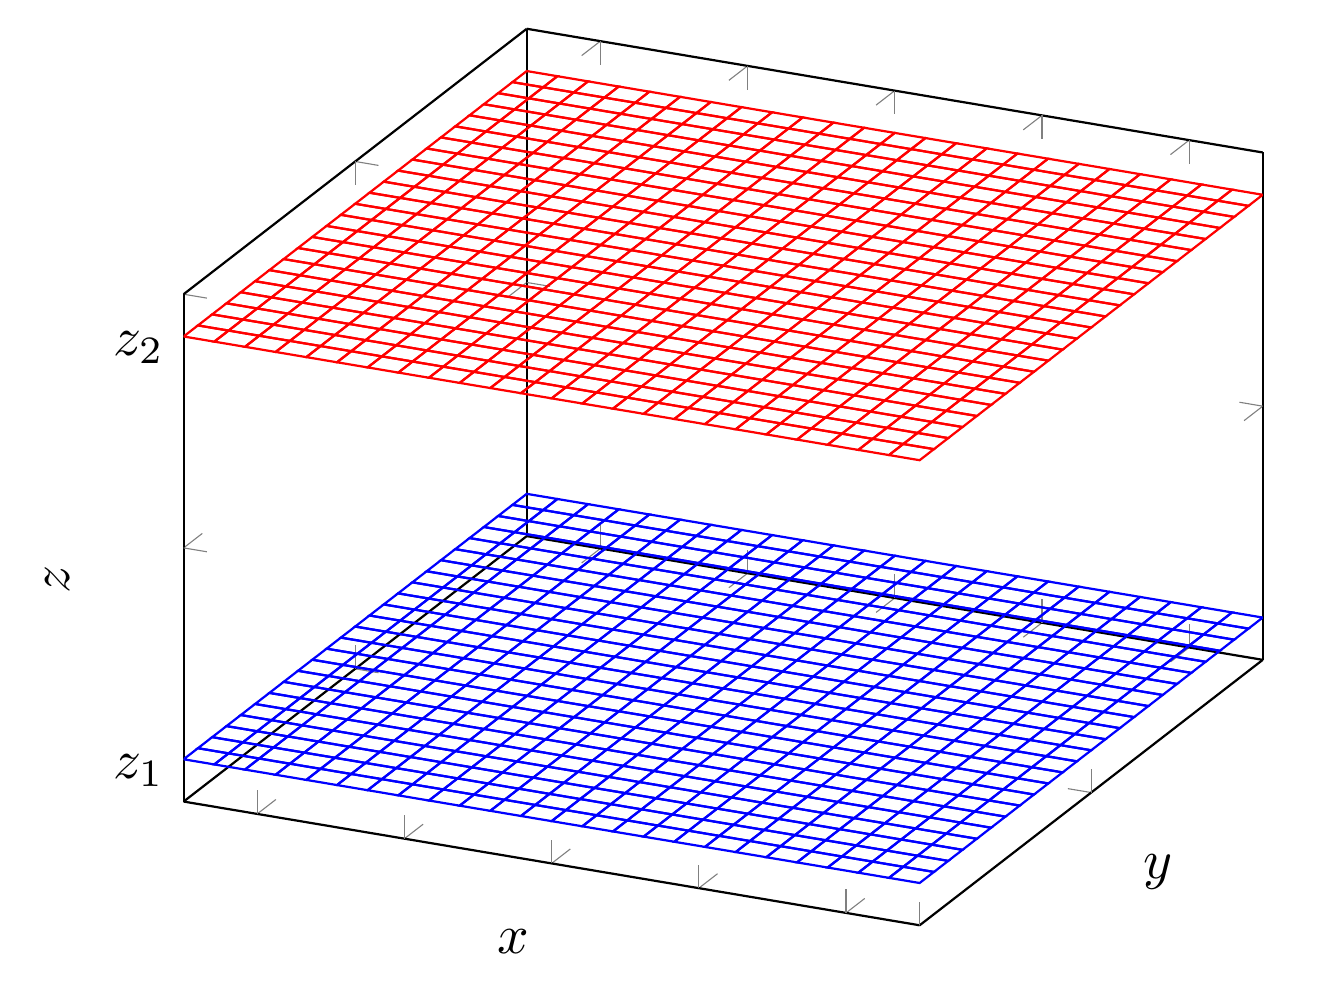
\begin{tikzpicture}[scale=2.0]
    \begin{axis}[
        xticklabels={,,},
        yticklabels={,,},
        zticklabels={$z_{2}$, ,$z_{1}$, ,$z_{2}$},
        zlabel=$z$,
        xlabel=$x$,
        ylabel=$y$
        ]
        \addplot3[mesh] {5};
        \addplot3[mesh] {7};
    \end{axis}
\end{tikzpicture}

% \begin{figure}
% \begin{tikzpicture}[scale=2.0]
%         \begin{axis}[
%         xticklabels={,,},
%         yticklabels={,,},
%         zticklabels={$z_{2}$,'',$z_{1}$,,$z_{2}$},
%         zlabel=$z$,
%         xlabel=$x$,
%         ylabel=$y$
%         ]
%             \addplot3[mesh] {5};
%             \addplot3[mesh] {7};
%         \end{axis}
% \end{tikzpicture}
% \caption{Se representan dos planos: sobre el plano azul hemos
% realizado las medidas del valor del campo en todos los puntos que
% son nodos de la rejilla y en el plano rojo se pretende inferir el
% campo a partir de las medidas en el plano azul. La separación entre
% nodos es de $\Delta x$ en la dirección $x$ y de $\Delta y$ en la
% dirección $y$}
% \end{figure}

\end{document}